\subsection{Basic Principle of Counting}

\begin{theorem}{Basic Principle of Counting}{basic-counting-principle}
  Suppose a first task can be performed in $m$ ways. Regardless of how the first task is performed, a second task can be performed in $n$ ways. Then both tasks can be performed in $mn$ ways.
\end{theorem}

The possible outcomes are ordered pairs:
\[
  \begin{array}{cccc}
    (1,1)  & (1,2)  & \cdots & (1,n)  \\
    (2,1)  & (2,2)  & \cdots & (2,n)  \\
    \vdots & \vdots & \ddots & \vdots \\
    (m,1)  & (m,2)  & \cdots & (m,n)
  \end{array}
\]

\begin{example}[Seating Students]
  How many arrangements are possible for $10$ students in a row of $10$ seats?
  \[
    \begin{array}{c|ccccc}
      \text{Seat number} & 1  & 2 & 3 & \cdots & 10 \\
      \text{Choices}     & 10 & 9 & 8 & \cdots & 1
    \end{array}
  \]
  By repeated application of \ref{thm:basic-counting-principle}, the total number of arrangements is
  \[
    10 \cdot 9 \cdot 8 \cdots 1 = 10!.
  \]
\end{example}

\subsection{Arrangements with Repeated Objects}

\begin{example}[Arranging MISSISSIPPI]
  How many distinguishable words can be formed using all the letters of \texttt{MISSISSIPPI}?

  Label the repeated letters:
  \[
    M,\ I_1,I_2,I_3,I_4,\ S_1,S_2,S_3,S_4,\ P_1,P_2.
  \]
  There are $11!$ arrangements of the labeled letters. Each word is counted $4!\,4!\,2!\,1!$ times, since permuting labels among identical letters leaves the word unchanged. Thus the number of distinguishable words is
  \[
    \frac{11!}{4!\,4!\,2!\,1!}.
  \]
\end{example}

\begin{theorem}{Arrangements with Repeated Objects}{repeated-object-arrangements}
  Suppose $n$ objects consist of $r$ distinct types, with $n_i$ identical objects of type $i$, where
  \[
    n_1+n_2+\cdots+n_r=n.
  \]
  The number of distinguishable arrangements is
  \[
    \frac{n!}{n_1!\,n_2!\cdots n_r!}
    = \binom{n}{n_1,n_2,\ldots,n_r}.
  \]
\end{theorem}

\subsection{Combinations}

\begin{example}[Choosing a Committee]
  How many $4$-person committees can be formed from a group of $10$ people?

  There are $10\cdot9\cdot8\cdot7$ ordered selections. Each committee is counted $4!$ times, so the number of committees is
  \[
    \frac{10\cdot9\cdot8\cdot7}{4!}
    = \frac{10!}{4!\,6!}
    = \binom{10}{6}
    = \binom{10}{4}.
  \]
\end{example}

To choose $k$ objects from $n$ distinct objects without replacement:
\[
  \begin{array}{c|cccc}
    \text{Selection number} & 1 & 2   & \cdots & k       \\
    \text{Choices}          & n & n-1 & \cdots & n-(k-1)
  \end{array}
\]
Each unordered selection occurs in $k!$ orders. Hence the number of selections is
\[
  \frac{n(n-1)\cdots(n-(k-1))}{k!}
  = \frac{n!}{k!\,(n-k)!}
  = \binom{n}{k}.
\]

\subsection{Binomial Theorems}

Recall that, for integers $0\le k\le n$,
\[
  \binom{n}{k}=\frac{n!}{k!\,(n-k)!}.
\]

\begin{theorem}{Binomial Theorem 1: Pascal's Identity}{pascal-identity}
  For integers $n\ge2$ and $1\le k\le n-1$,
  \[
    \binom{n}{k}=\binom{n-1}{k}+\binom{n-1}{k-1}.
  \]
\end{theorem}

\begin{proof}
  Count the $k$-element subsets of $\{1,2,\ldots,n\}$ by whether they contain $1$.
  \begin{itemize}
    \item If $1$ is included, choose the remaining $k-1$ elements in $\binom{n-1}{k-1}$ ways.
    \item If $1$ is excluded, choose all $k$ elements in $\binom{n-1}{k}$ ways.
  \end{itemize}
  These cases are exhaustive and mutually exclusive, so their counts add.
\end{proof}

\subsubsection{Pascal's Triangle}

The rows of Pascal's triangle list the binomial coefficients. By Theorem~\ref{thm:pascal-identity}, each interior entry is the sum of the two entries above it.

\begin{center}
  \begin{tikzpicture}[x=0.7cm,y=0.65cm]
    \foreach \row/\col/\value in {0/0/1,1/0/1,1/1/1,2/0/1,2/1/2,2/2/1,3/0/1,3/1/3,3/2/3,3/3/1,4/0/1,4/1/4,4/2/6,4/3/4,4/4/1}
      \node at ({2*\col-\row},-\row) {$\value$};
    \node at (0,-5) {$\cdots$};
  \end{tikzpicture}
  \qquad
  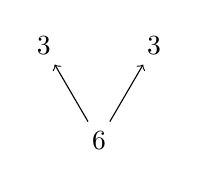
\begin{tikzpicture}[baseline]
    \node (left) at (0,0) {$3$};
    \node (right) at (1.4,0) {$3$};
    \node (sum) at (0.7,-1.2) {$6$};
    \draw[->] (sum) -- (left);
    \draw[->] (sum) -- (right);
  \end{tikzpicture}
  \qquad
  $\displaystyle\binom{3}{2}+\binom{3}{1}=\binom{4}{2}$
\end{center}

\begin{example}[Binomial Expansions]
  \begin{align*}
    (x+y)^2 & = \binom{2}{2}x^2+\binom{2}{1}xy+\binom{2}{0}y^2,                    \\
    (x+y)^3 & = \binom{3}{3}x^3+\binom{3}{2}x^2y+\binom{3}{1}xy^2+\binom{3}{0}y^3.
  \end{align*}
\end{example}

\subsubsection{The Binomial Expansion}

\begin{theorem}{Binomial Theorem 2: Binomial Expansion}{binomial-expansion}
  For every integer $n\ge0$,
  \[
    (x+y)^n=\sum_{k=0}^n\binom{n}{k}x^k y^{n-k}.
  \]
\end{theorem}

\begin{proof}
  The case $n=0$ is immediate. For $n=1$,
  \[
    (x+y)^1=\binom{1}{1}x+\binom{1}{0}y.
  \]
  Suppose the formula holds for $n-1$:
  \[
    (x+y)^{n-1}=\sum_{k=0}^{n-1}\binom{n-1}{k}x^k y^{n-1-k}.
  \]
  Multiplying by $x+y$ gives
  \begin{align*}
    (x+y)^n
     & = (x+y)\sum_{k=0}^{n-1}\binom{n-1}{k}x^k y^{n-1-k} \\
     & = \sum_{k=0}^{n-1}\binom{n-1}{k}x^{k+1}y^{n-(k+1)}
    +\sum_{k=0}^{n-1}\binom{n-1}{k}x^k y^{n-k}.
  \end{align*}
  Set $j=k+1$ in the first sum and $j=k$ in the second:
  \begin{align*}
    (x+y)^n
     & = \sum_{j=1}^{n}\binom{n-1}{j-1}x^j y^{n-j}
    +\sum_{j=0}^{n-1}\binom{n-1}{j}x^j y^{n-j}                                           \\
     & = x^n+\sum_{j=1}^{n-1}\binom{n-1}{j-1}x^j y^{n-j}
    +y^n+\sum_{j=1}^{n-1}\binom{n-1}{j}x^j y^{n-j}                                       \\
     & = x^n+y^n+\sum_{j=1}^{n-1}\left[\binom{n-1}{j-1}+\binom{n-1}{j}\right]x^j y^{n-j} \\
     & = x^n+y^n+\sum_{j=1}^{n-1}\binom{n}{j}x^j y^{n-j}                                 \\
     & = \sum_{j=0}^n\binom{n}{j}x^j y^{n-j}
    = \sum_{k=0}^n\binom{n}{k}x^k y^{n-k}.
  \end{align*}
  The fourth equality uses Theorem~\ref{thm:pascal-identity}.
\end{proof}

\subsubsection{Sums of Binomial Coefficients}

\begin{theorem}{Binomial Theorem 3: Binomial Sums}{binomial-sums}
  For every integer $n\ge0$,
  \[
    \sum_{k=0}^n\binom{n}{k}=2^n.
  \]
  For every integer $n\ge1$,
  \[
    \sum_{k=0}^n(-1)^k\binom{n}{k}=0.
  \]
\end{theorem}

\begin{proof}
  In Theorem~\ref{thm:binomial-expansion}, take $x=y=1$ for the first identity and $x=-1$, $y=1$ for the second.
\end{proof}

\subsection{The Multinomial Theorem}

\begin{theorem}{Multinomial Theorem}{multinomial-theorem}
  For integers $n\ge0$ and $r\ge1$,
  \[
    (x_1+\cdots+x_r)^n
    =\sum_{\substack{n_1+\cdots+n_r=n\\n_i\ge0\text{ integers}}}
    \binom{n}{n_1,n_2,\ldots,n_r}x_1^{n_1}x_2^{n_2}\cdots x_r^{n_r},
  \]
  where
  \[
    \binom{n}{n_1,n_2,\ldots,n_r}=\frac{n!}{n_1!\,n_2!\cdots n_r!}.
  \]
\end{theorem}

\begin{proof}
  Expanding the product of $n$ factors, a term $x_1^{n_1}\cdots x_r^{n_r}$ results from choosing $x_i$ from exactly $n_i$ factors for each $i$.

  Its coefficient counts the ways to divide the $n$ factor positions into $r$ labeled groups of sizes $n_1,\ldots,n_r$. By Theorem~\ref{thm:repeated-object-arrangements}, this count is
  \[
    \binom{n}{n_1,n_2,\ldots,n_r}.
  \]
  Summing over all nonnegative integer choices with $n_1+\cdots+n_r=n$ gives the expansion.
\end{proof}
